\section{Parcial con respecto a los pesos en la penúltima capa}

\begin{figure}[h]
 \centering
 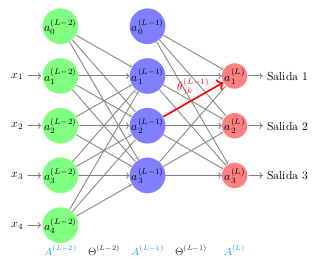
\includegraphics[scale=0.5]{../Figuras/AredNa.png}
 %\caption{Penúltima capa.}
 \label{fig:graficaLog}
\end{figure}

Una vez más para ser más legible los cálculos vamos a comenzar a calcular el gradiente considerando que ahorita solamente estamos evaluando a la red en un ejemplo y vamos a tener que resolverlo por etapas lo que estamos pensando es lo siguiente nuestra función de la red neuronal como aquí las entradas produjo aquí las etiquetas correspondientes y ahora lo que nuestra función de errores están viviendo es la distancia entre lo que obtuvimos en esta capa y una colección de etiquetas que era lo que nosotros queríamos que saliera entonces nuestra función de error está actuando directamente sobre esta capa nada más pero cómo se llegó a este resultado bueno pues se llegó después de haber realizado cálculos sobre lo que teníamos evaluar acá utilizando los pesos en esta capa cómo se llegó este resultado pues habiendo evaluado lo que había ocurrido acá involucrando también a los pesos de esta otra capa entonces podemos pensar que los valores que obtuvimos aquí a la salida dependen de los pesos en cada una de las capas sin embargo la dependencia es ligeramente distinta en el sentido de que la distancia entre este peso y este es inmediata aquí para poder saber cómo depende este resultado final de un peso que tengo acá atrás pues tengo que irme dos niveles más hacia acá recordando que este influyó en el cálculo de este número entonces el gradiente lo vamos a ir calculando cappa porque de ahí viene precisamente el nombre de bach preparation entonces lo primero y lo más sencillo va a ser calcular como dependió la función de error de los pesos que se encuentran inmediatamente detrás de las neuronas de salida y así verdad necesito explicar poco a poco la anotación lo que vamos a hacer en este momento es considerar que en el algoritmo feedforward la primera capa la vamos a tomar con los índices y la siguiente capa índices j la tercera capa índices k por eso estamos pensando que los pesos de la última capa conectan a la neurona j con la neurona k pero para considerar que vamos a ir haciendo esto en reversa nos importa que esta es la última capa no le vamos a llamar la capa l y luego vamos a trabajar con la capa anterior que sería la capa l menos 1 luego vamos a ir a la capa todavía anterior l menos 2 y esta anotación también nos va a permitir darnos cuenta que si hubiera más capas hacia atrás pues siempre y sencillamente iríamos restando más números otro punto importante en la anotación vamos a asignarle a los pesos el índice correspondiente a la capa anterior a la cual tuvieron que multiplicar entonces cada capa va asociada con el bloque de pesos que tiene adelante el cálculo final entonces para la capa l depende de los valores de activación en la capa l - sólo x los pesos en la matriz l menos 1 y así obtenemos lo que está en la campaña memorizar a la anotación porque la vamos a necesitar o bien entonces lo que tenemos en esta línea inmediatamente es la función de error observen que quite ahorita la suma sobre los diferentes ejemplares de entrenamiento por eso solamente lo vamos a calcular para un ejemplar y al resto al ratito ya será sencillo generalizar a varios ejemplares bien entonces si tenemos un suelo ejemplar de entrenamiento lo que si nos sigue importando es el hecho de que tenemos varias clases de entre las cuales podría haber estado la respuesta y por eso tenemos la suma desde que hay igual a 1 hasta SL. 
Entonces a través un poco de notación s l es el número de neuronas que tenemos en la capa l s l menos 1 sería el número de neuronas en la capa l menos suelo y así sucesivamente y aquí viene la misma definición que ya teníamos antes el valor que queremos llegar y el valor que realmente obtuvimos de hecho podemos quitar ahorita este 6 porque solamente hay un ejemplar de entrenamiento entonces ya tenemos aquí un solo ejemplo y ahora lo que queremos hacer es calcular la derivada con respecto a los pesos justamente antes de haber evaluado el valor de la última capa la notación que estamos utilizando aquí en vez de la h de hipótesis es el hecho de que tal cual el valor de la hipótesis es el valor de activación de la neurona entonces estamos hablando del valor de activación de cada una de estas y esas son las áreas si se fijan cuando evaluamos el algoritmo feedforward ya obtuvimos los valores de activación de hecho de todas las neuronas entonces los podemos utilizar aquí y precisamente lo que vamos a hacer para poder calcular la derivada es recordar hecho eso de nuestro valor de activación fue calculado con las reglas de activación de un perceptor entonces comenzamos a calcular la derivada de la entropía cruzada en primer lugar vamos a observar que estoy calculando la parcial del error con respecto a uno de los pesos bueno aquí tenemos la suma sobre todo de las neuronas de salida no pero observemos qué ocurre con este peso solamente está contribuyendo a la salida de esta neurona a esta neurona no le afecta en lo más mínimo lo que haya ocurrido aquí y esta neurona tampoco le afecta luego entonces la parcial de estos dos elementos con respecto a este peso vale cero porque no hay una dependencia son constantes en este caso si para la neurona que está conectada con este peso es decir la neurona acá sí importa lo que ocurrió con este peso por ello de los tres elementos que teníamos aquí aparece en el dibujo es el en general solamente va a sobrevivir uno de los términos y es aquel donde estamos trabajando exactamente con la neurona carísima entonces si de momento ya no tenemos esta suma podemos trabajar solamente con lo que hay aquí adentro tenemos nuestro signo menos acá afuera después llegué acá 1 - que realmente son constantes entonces aquí sale la aie de acá la derivada del logaritmo es 1 entre lo que está dentro del logaritmo por eso tenemos aquí acá en el denominador regla de la cadena derivada de lo de adentro entonces tenemos otra vez la derivada con respecto a z jk del valor de activación acá y aquí es importante que recordemos cómo era calculado este valor y era precisamente con la función de activación aplicada sobre la combinación lineal de todos los pesos que venían desde la capa anterior y que nos conectaban con este valor y estaban multiplicados pues por los valores de activación precisamente de la capa anterior es decir estamos considerando que esta neurona tiene las contribuciones de todas estas neuronas de acá y entrando para acá y eso es lo que estamos escribiendo aquí de manera explícita igualmente este es un término que ya habíamos calculado para poder evaluar el fit forward las setas que son las combinaciones lineales de las valores de activación de atrás por los peces entonces si recordamos eso podemos simplificar nos un poco la nota y haciendo lo mismo con este otro término otra vez tenemos este que es una constante después la derivada del logaritmo 1 entre lo de acá por la derivada parcial de lo que esté aquí adentro la deriva de parcial de 1 pues va a ser un 0 de este menos lo sacamos y lo estamos poniendo aquí dejamos indicado de momento la derivada parcial de aquí tenemos estoy escribiendo en versión resumida lo mismo que tenemos acá porque es exactamente bien ahora si observamos este elemento otra vez podemos aprovechar el hecho de que solamente nos interesa este peso entonces realmente lo que ocurre con estas otras dos neuronas de momento no nos está afectando solamente nos interesa el valor de a que conecta con este esa jota exactamente los 102 las fotos primas que tenemos aquí solamente nos vamos a quedar con esto si hacemos eso entonces ya no necesitamos considerar aquí toda la zona para el siguiente término es el que me falta por aquí es decir calculé la derivada parcial de todo lo que estaba acá adentro con respecto a z acá pero pues ahora que calculemos la derivada pues vamos a tener que seguir pues entonces como se va a ver esto en primer lugar este término se copia tal y como está el menos aquí lo seguimos cargando que habíamos visto anteriormente acerca de la derivada de la función logística 
Pues que es la función logística por 1 - ella misma es esa primera parte la vamos a dejar aquí indicada por otro lado tenemos que continuar con la regla de la cadena calculando la derivada de esta suma que tenemos aquí adentro pero lo que acabamos de ver es que solamente va a sobrevivir pues el elemento donde jota prima es jota y los otros se van a morir son constantes con respecto a este peso entonces la derivada de este elemento con respecto a éste es uno y el término que queda sobreviviendo es esta y es precisamente entonces le estoy poniendo aquí afuera de una vez porque nos va a salir otro idéntico del lado derecho recuerdan de la x que teníamos cuando calculamos la deriva de la signo y bueno aquí está precisamente el término que está sobreviviendo muy bien entonces repitiendo la misma idea de este lado tenemos el mismo factor tenemos que prima y también aquí al aplicar la regla de la cadena va a salir una idénticamente entonces por eso le estaba factor izando de una vez lo siguiente que vamos a hacer es bueno factorizar este también lo estamos poniendo aquí afuera y otra vez lo que vamos a hacer es trabajar con estos dos para tratar de escribirlos de una manera más amigable ponemos entonces como un denominador estos dos se multiplican este que está aquí lo multiplicó por el denominador de acá estoy acá lo multiplicó por el de acá tenemos el signo menos los voy a llegar por 1 menos acá menos acá por un número chica una vez que hacemos esto las cosas se vuelven hermosas esto de aquí es rica esto de acá es un término cruzado allí - una al menos por menos más un término cruzado allí éste se va con éste. 
Ahora tenemos que recordar también que propiedad bonita tenía la derivada prima pues era g por uno menos 100 pero la función g evaluada en la combinación lineal que es pues es exactamente la que calculamos cuando estábamos haciendo el fit for work así salió entonces este es que es que tengo aquí le sustituyó simple y sencillamente por la sas que fue lo que calculamos en el instante en el que recuerdo esto o miren esteban y fue los que nos quedó entonces pues únicamente la diferencia entre lo que quería y lo que salió multiplicado por el valor de activación de la neurona en la capa anterior bien porque es bonito ser entropía cruzada consigo les basta con legis ticas muy bien entonces a esto que esté aquí se le acostumbra poner el nombre del está acá porque podemos decir que fue el error que se cometió en la última capa y aquí quedó bastante literal simplemente tomamos lo que salió bueno lo que queríamos - lo que salió este elemento que está acá es lo que está contribuyendo precisamente el hecho de que este peso no se estaba conectando con alguien en la parte de atrás y ya tenemos entonces la manera de calcular todas las parciales del error con respecto a los pesos y en esta capa vamos a ver entonces en el próximo capítulo cómo calcular las derivadas con respecto a los pesos que están en la capacidad.
